\section{Unified Modeling Language (UML)}

\hspace{1cm} The Unified Modeling Language (UML) is a graphical language for 
visualizing, specifying, constructing, and documenting software-intensive systems. 
This language is maintained by the Object Management Group (OMG) \cite{UML}.

UML is one of the most widely used modeling languages for describing real-world 
application domains. It works with various object and component methods to represent 
software systems. As software systems grow in size, complexity, and distribution, 
building and maintaining them becomes more challenging. UML helps reduce this 
complexity by providing a high level of abstraction that captures essential 
information needed for designing and developing software systems.

UML includes multiple diagram types, each focusing on different aspects of a design. 
These diagrams fall into two main categories: (1) structural diagrams that represent 
the static aspects of a system, and (2) behavioral diagrams that describe the dynamic 
aspects. These structural and behavioral categories collectively contain fourteen 
different diagram types, as specified in the UML Reference Manual \cite{UML_Reference_Manual}.

For this thesis, two related structural diagrams are particularly relevant and will be presented in the following subsections: class diagrams, which define the abstract structure of a system, and object diagrams, which provide concrete instances of that structure.

%%% Sample
% The Unified Modeling Language (UML) is a graphical language for 
% visualizing, specifying, constructing, and documenting software-intensive systems.
% This unified language is maintained by the Object Management Group (OMG) [58].
% The UML has become one of the most widely used modeling language that can
% be used with all significant object and component methods for describing real-world
% application domains. Software systems, in today’s world, are growing in size, complex
% ity, distribution and importance. As a result, building and maintenance of software
% have become a more complex and challenging task. Therefore, the deployment of
% languages such as UML reduces the complexity and difficulty by providing a high
% level of abstraction, which describes precise and essential information for designing
% and developing the software system [50].  
% The graphical representation of the UML includes a set of diagrams, each focusing
% on different aspects of a design. The UML Notation Guide states all the notation of 
% diagram elements [58]. These diagrams can be classified into two groups (a) a structural
% diagram that represents the static aspect of the system, and (b) a behavioral diagram
% that describes the dynamic aspect of the system. Altogether, fourteen different model
% types can be found in the Unified Modeling Language Reference Manual [71]. In this
% thesis, two diagrams, i.e., class diagram and object diagram, have
% been extensively used and are explained further in this section.

\subsection{Class Diagram}
Class diagrams are the foundation of structural modeling in UML and the most widely 
used diagram type in object-oriented systems. They illustrate the static structure 
of a system by depicting classes, their attributes, operations, and the relationships 
between classes. These concepts can be observed in Figure \ref{fig:class_diagram_bank_account_model}, 
which shows a class diagram of a simple bank account system.

\begin{figure}
    \begin{center}
        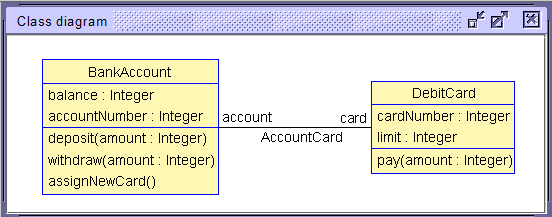
\includegraphics[width=0.8\textwidth]{figures/c1/BankAccount/BankAccount_ClassDiagram.png}
        \caption{Class diagram of the Bank Account Model.}
        \label{fig:class_diagram_bank_account_model}
    \end{center}
\end{figure}

In this diagram, we see two classes, \texttt{BankAccount} and \texttt{DebitCard}, 
which represent sets of objects that share common characteristics. Each class 
contains attributes that describe the data values their objects may contain. 
The \texttt{BankAccount} class has attributes such as:
\begin{itemize}
    \item \texttt{accountNumber}: a unique identifier for the bank account
    \item \texttt{balance}: the current balance of the bank account
\end{itemize}
Similarly, the \texttt{DebitCard} class has attributes:
\begin{itemize}
    \item \texttt{cardNumber}: a unique identifier for the debit card
    \item \texttt{limit}: the maximum amount that can be withdrawn using the debit card
\end{itemize}

Classes also include operations that specify the behaviors objects can perform. 
In our example, the \texttt{BankAccount} class defines three operations:
\begin{itemize}
    \item \texttt{deposit(amount)}: adds the specified amount to the account balance
    \item \texttt{withdraw(amount)}: deducts the specified amount from the balance
    \item \texttt{assignNewCard()}: creates and assigns a new debit card to the bank account
\end{itemize}
These operations represent the functional capabilities of \texttt{BankAccount} objects, 
defining how they can interact with other objects and how their state can change over 
time. While attributes describe what an object knows, operations describe what an 
object can do.

Relationships between these classes are represented by the \texttt{AccountCard} 
association, which connects \texttt{BankAccount} and \texttt{DebitCard}. 
Multiplicity indicators on this association would show how many objects of one class 
can be linked to objects of another class. In addition to simple associations like 
this one, class diagrams can include more specialized relationship types: aggregation 
and composition (both representing whole-part relationships with different levels of 
dependency), and generalization (inheritance relationships where specialized classes 
inherit properties from a general class).

Class diagrams represent the static structure of a system at a particular point in 
time, providing the vocabulary and structural framework that other diagrams and 
behavioral specifications build upon.

%%% Version 3
% Class diagrams are the foundation of structural modeling in UML and the most widely used diagram type in object-oriented systems. They illustrate the static structure of a system by depicting classes, their attributes, operations, and the relationships between classes. These concepts can be observed in Figure \ref{fig:class_diagram_bank_account_model}, which shows a class diagram of a simple bank account system.

% \begin{figure}
%     \begin{center}
%         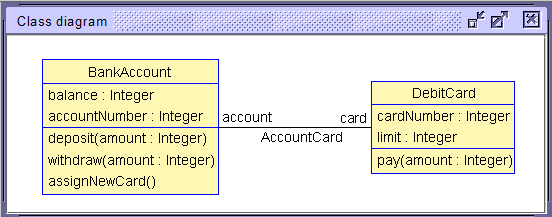
\includegraphics[width=0.8\textwidth]{figures/c1/BankAccount/BankAccount_ClassDiagram.png}
%         \caption{Class diagram of the Bank Account Model.}
%         \label{fig:class_diagram_bank_account_model}
%     \end{center}
% \end{figure}

% In this diagram, we see two classes, BankAccount and DebitCard, which represent sets of objects that share common characteristics. Each class contains attributes that describe the data values their objects may contain. The BankAccount class has attributes such as:
% \begin{itemize}
%     \item accountNumber: a unique identifier for the bank account
%     \item balance: the current balance of the bank account
% \end{itemize}

% Similarly, the DebitCard class has attributes:
% \begin{itemize}
%     \item cardNumber: a unique identifier for the debit card
%     \item limit: the maximum amount that can be withdrawn using the debit card
% \end{itemize}

% Classes also include operations that specify the behaviors objects can perform. In our example, the BankAccount class defines three operations:
% \begin{itemize}
%     \item deposit(amount): adds the specified amount to the account balance
%     \item withdraw(amount): deducts the specified amount from the balance
%     \item assignNewCard(): creates and assigns a new debit card to the bank account
% \end{itemize}
% These operations represent the functional capabilities of BankAccount objects, defining how they can interact with other objects and how their state can change over time. While attributes describe what an object knows, operations describe what an object can do.
% The relationship between these classes is represented by the AccountCard association, which connects BankAccount and DebitCard. Multiplicity indicators on this association would show how many objects of one class can be linked to objects of another class. In addition to simple associations like this one, class diagrams can include more specialized relationship types: aggregation and composition (both representing whole-part relationships with different levels of dependency), and generalization (inheritance relationships where specialized classes inherit properties from a general class).
% Class diagrams represent the static structure of a system at a particular point in time, providing the vocabulary and structural framework that other diagrams and behavioral specifications build upon.

\subsection{Object Diagram}
Object diagrams are structural diagrams that represent real-world entities or 
modeled system elements as concrete instances of classes. While class diagrams 
show abstract structures, object diagrams provide snapshots of a system at specific 
points in time, showing actual objects with specific attribute values and the links 
connecting them.

\begin{figure}
    \begin{center}
        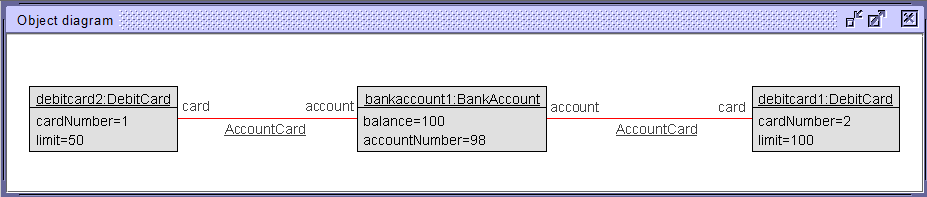
\includegraphics[width=0.8\textwidth]{figures/c1/BankAccount/BA_ObjectDiagram.png}
        \caption{Object diagram of the Bank Account Model.}
        \label{fig:object_diagram_bank_account_model}
    \end{center}
\end{figure}

Figure \ref{fig:object_diagram_bank_account_model} shows an example object diagram for the banking system previously described in the class diagram (Figure \ref{fig:class_diagram_bank_account_model}).
The links between objects in the diagram represent instances of the associations defined in the class diagram. Here, the \texttt{AccountCard} links connect the \texttt{bankaccount1} object to both debit card objects, showing that this particular bank account has two associated debit cards with different withdrawal limits.

Object diagrams provide concrete examples that help verify that a system model behaves as expected. They are valuable for validating class structures, illustrating complex relationships, and demonstrating specific scenarios during system design. While object diagrams excel at representing static information about system states, they do not capture the dynamic interactions that cause state changes. This characteristic defines both the strength and scope of object diagrams within UML modeling - they offer precise snapshots of system state at a particular moment in time, complementing the abstract structural representations provided by class diagrams.

%%% Version 2
% Object diagrams are structural diagrams that represent real-world entities or 
% modeled system elements as concrete instances of classes. While class diagrams 
% show abstract structures, object diagrams provide snapshots of a system at specific 
% points in time, showing actual objects with specific attribute values and the links 
% connecting them [77].

% Objects in these diagrams are instances of classes defined in the class diagram, 
% with concrete values assigned to their attributes. Links between objects are 
% instances of the associations defined in the class diagram. This concrete 
% representation makes object diagrams particularly valuable for verification purposes.

% % Example here
% \begin{figure}
%     \begin{center}
%         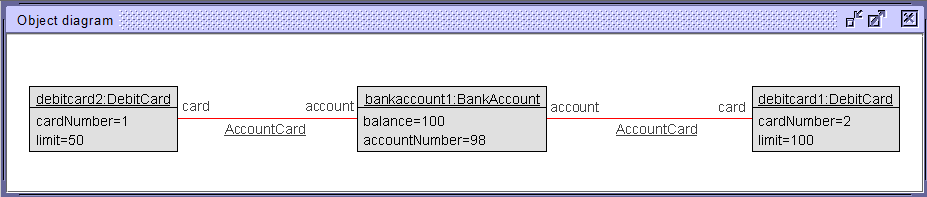
\includegraphics[width=0.8\textwidth]{figures/c1/BankAccount/BA_ObjectDiagram.png}
%         \caption{Object diagram of the Bank Account Model.}
%         \label{fig:object_diagram_bank_account_model}
%     \end{center}
% \end{figure}

% Figure \ref{fig:object_diagram_bank_account_model} shows the example object diagram, where debitcard1 and debitcard2 
% objects are instances of the class DebitCard, and bankaccount1 object is the instance of the
%  class BankAccount from the class diagram shown in Fig. \ref{fig:class_diagram_bank_account_model}. 
%  Between debitcard1, debitcard2 and bankaccount1, there exists the link AccountCard. 

% An important limitation of object diagrams is that they represent only a single 
% state of the system. When the system state changes through operation calls, 
% previous state information is lost. A single object diagram cannot represent 
% the flow of information or system evolution over time. This limitation is 
% particularly relevant to our work, as it highlights why standard UML/OCL approaches 
% struggle with temporal specifications. In this thesis, object diagrams play a crucial 
% role in our validation approach, where sequences of object diagrams (filmstrips) 
% are used to represent and verify temporal properties.

% These diagrams form the foundation of object-oriented modeling and are essential 
% for understanding the system structure that our temporal and event-based extensions 
% will work with. In this thesis, class diagrams provide the structural framework 
% upon which temporal properties will be defined and verified.